
\section{Methodology}
\subsection{Preliminary}
\textbf{Latent Video Diffusion Model~(LVDM).} The LVDM enhances the stable diffusion model~\cite{ramesh2022hierarchical} by integrating a 3D UNet, thereby empowering efficient video data processing. This 3D UNet design augments each spatial convolution with an additional temporal convolution and follows each spatial attention block with a corresponding temporal attention block. It is optimized by employing a noise-prediction objective function:
\begin{equation}
    l_\epsilon = ||\epsilon - \epsilon_\theta(z_t, t, c)||^2_2,
    \label{eq:training_objective}
\end{equation}
Here, $\epsilon_\theta(\cdot)$ signifies the 3D UNet's noise prediction function. The condition 
$c$ is guided into the UNet using cross-attention for adjustment. Meanwhile, $z_t$ denotes the noisy hidden state, evolving like a Markov chain that progressively adds Gaussian noise to the initial latent state $z_0$:
\begin{equation}
    z_t=\sqrt{\bar{\alpha}_t}z_0 + \sqrt{1 - \bar{\alpha}_t}\epsilon, \quad\epsilon \sim \mathcal{N}(0, I),
    \label{eq:add_noise}
\end{equation}
where $\bar{\alpha}_t = \prod_{i=1}^t(1-\beta_t)$ and $\beta_t$ is a coefficient that controls the noise strength in step $t$.


\noindent \textbf{Diffusion Transformer~(DiT).} The DiT~\cite{peebles2023scalable} introduces a novel architecture that merges the strengths of diffusion models with transformer architectures~\cite{DBLP:conf/nips/VaswaniSPUJGKP17}.  This integration aims to address the limitations of traditional UNet-based latent diffusion models (LDMs), improving their performance, versatility, and scalability. While keeping the overall framework consistent with existing LDMs, the key shift lies in replacing the UNet with a transformer architecture for learning the denoising function $\epsilon_\theta(\cdot)$, thereby marking a pivotal advance in the realm of generative modeling.

%While maintaining the overarching formulation congruent with established LDM frameworks, the paradigm shift resides in the substitution of the U-Net with a transformer architecture for the denoising function $\epsilon_\theta(\cdot)$ learning, thereby marking a pivotal advance in the realm of generative modeling.

\subsection{Tora}
Tora employs the Spatial-Temporal Diffusion Transformer (ST-DiT) from OpenSora as its foundational model. To facilitate user-friendly motion control while aligning with the scalability of DiT, Tora integrates two novel motion-processing components: the Trajectory Extractor (TE) and the Motion-guidance Fuser (MGF). An overview of Tora's workflow is illustrated in Figure~\ref{fig:3}.

\noindent \textbf{Spatial-Temporal DiT.} The ST-DiT architecture incorporates two distinct block types: the Spatial DiT Block (S-DiT-B) and the Temporal DiT Block (T-DiT-B), arranged in an alternating sequence. The S-DiT-B comprises two attention layers, each performing Spatial Self-Attention (SSA) and Cross-Attention sequentially, succeeded by a point-wise feed-forward layer that serves to connect adjacent T-DiT-B block. Notably, the T-DiT-B modifies this schema solely by substituting SSA with Temporal Self-Attention (TSA), preserving architectural coherence. Within each block, the input, upon undergoing normalization, is concatenated back to the block's output via skip-connections. By leveraging the ability to process variable-length sequences, the denoising ST-DiT can handle videos of variable durations.

During processing, a video autoencoder~\cite{yu2023magvit} is first employed to diminish both spatial and temporal dimensions of videos. To elaborate, it encodes the input video $X \in \mathbb{R}^{L \times H \times W \times 3}$ into video latent $z_{0} \in \mathbb{R}^{l \times h \times w \times 4}$, where $L$ denotes the video length and $l = L / 4, h = H / 8, w = W / 8$.  $z_{0}$ is next ``patchified", resulting in a sequence of input tokens $I \in \mathbb{R}^{l \times s \times d} $. Here, $s = hw/p^2$ and $p$ denotes the patch size. 
%$I$ is then forwarded to the ST-DiT, which models these compressed representations. 
In both SSA and TSA, standard Attention is performed using Query ($Q$), Key ($K$), and Value ($V$) matrices:
\vspace{-2mm}
\begin{equation}
Q = W_{Q} \cdot I_\mathrm{norm}; K = W_{K} \cdot I_\mathrm{norm}; V = W_{V} \cdot I_\mathrm{norm},
\end{equation}
Here, $I_\mathrm{norm}$ is the normalized $I$, $W_{Q},W_{K}, W_{V}$ are learnable matrices.
The textual prompt is embedded with a T5 encoder and integrated using a cross-attention mechanism.
%The cross-attention mechanism is employed between the embedded prompt and the intermediate features from either the SSA or the TSA.

\noindent \textbf{Trajectory Extractor.} Trajectories have proven to be a more user-friendly method for controlling the motion of generated videos. Specifically, given a trajectory $traj=\left \{ (x_i, y_i) \right \} _{i=0}^{L-1} $, where $(x_i, y_i)$ denotes the spatial position $(x, y)$ at the $i$-$th$ frame the trajectory passes through. Previous studies primarily encode the horizontal offset $u(x_i,y_i)$ and the vertical offset $v(x_i,y_i)$ as the motion condition: 
\begin{equation}
u(x_i,y_i)= x_{i+1} - x_{i}; ~ v(x_i,y_i)= y_{i+1} - y_{i},
\end{equation}
However, the DiT model employs a video autoencoder and a patchification process to convert the video into patches. Here, each patch is derived across multiple frames, rendering it inappropriate to straightforwardly employ frame-to-frame offsets. To address this, our TE converts the trajectory into motion patches, which inhabit the same latent space as the video patches. Particularly, we begin by transforming the $traj$ into a trajectory map $g \in \mathbb{R}^{L \times H \times W \times 2}$, enhanced with a Gaussian Filter to mitigate scatter. Notably, the first frame employs a fully-zero map. Afterward, the trajectory map $g$ is translated into the RGB color space, producing $g_{vis} \in \mathbb{R}^{L \times H \times W \times 3}$ through a flow visualization technique. We use a 3D VAE to compress trajectory maps, achieving an 8x spatial and 4x temporal reduction, aligning with OpenSora framework. Our VAE is based on the MAGVIT-v2 architecture, with spatial compression initialized using the VAE of SDXL~\cite{DBLP:journals/corr/abs-2307-01952} to accelerate convergence. We train the model using reconstruction loss to obtain the compact motion latent representation $g_{m} \in \mathbb{R}^{l \times h \times w \times 4}$ from the $g_{vis}$.

To match the size of the video patches, we use the same patch size on 
$g_{m}$ and encode it using a series of convolutional layers, resulting in spacetime motion patches $f \in \mathbb{R}^{l \times s\times d' }$. Here $d'$ is the dimension of motion patches. The output of each convolutional layer is skip-connected to the input of the next layer to extract multi-level motion features:
\begin{equation}
f_i= \mathrm{Conv}^{i}~(f_{i - 1}) + f_{i - 1},
\end{equation}
where $f_i$ is the motion condition for $i$-$th$ ST-DiT block. 




\noindent \textbf{Motion-guidance Fuser.} To incorporate DiT-based video generation with the trajectory, we explore three variants of fusion architectures that inject motion patches into each ST-DiT block. These designs are illustrated in Figure~\ref{fig:4}.

\begin{figure}[!t]
    \centering
    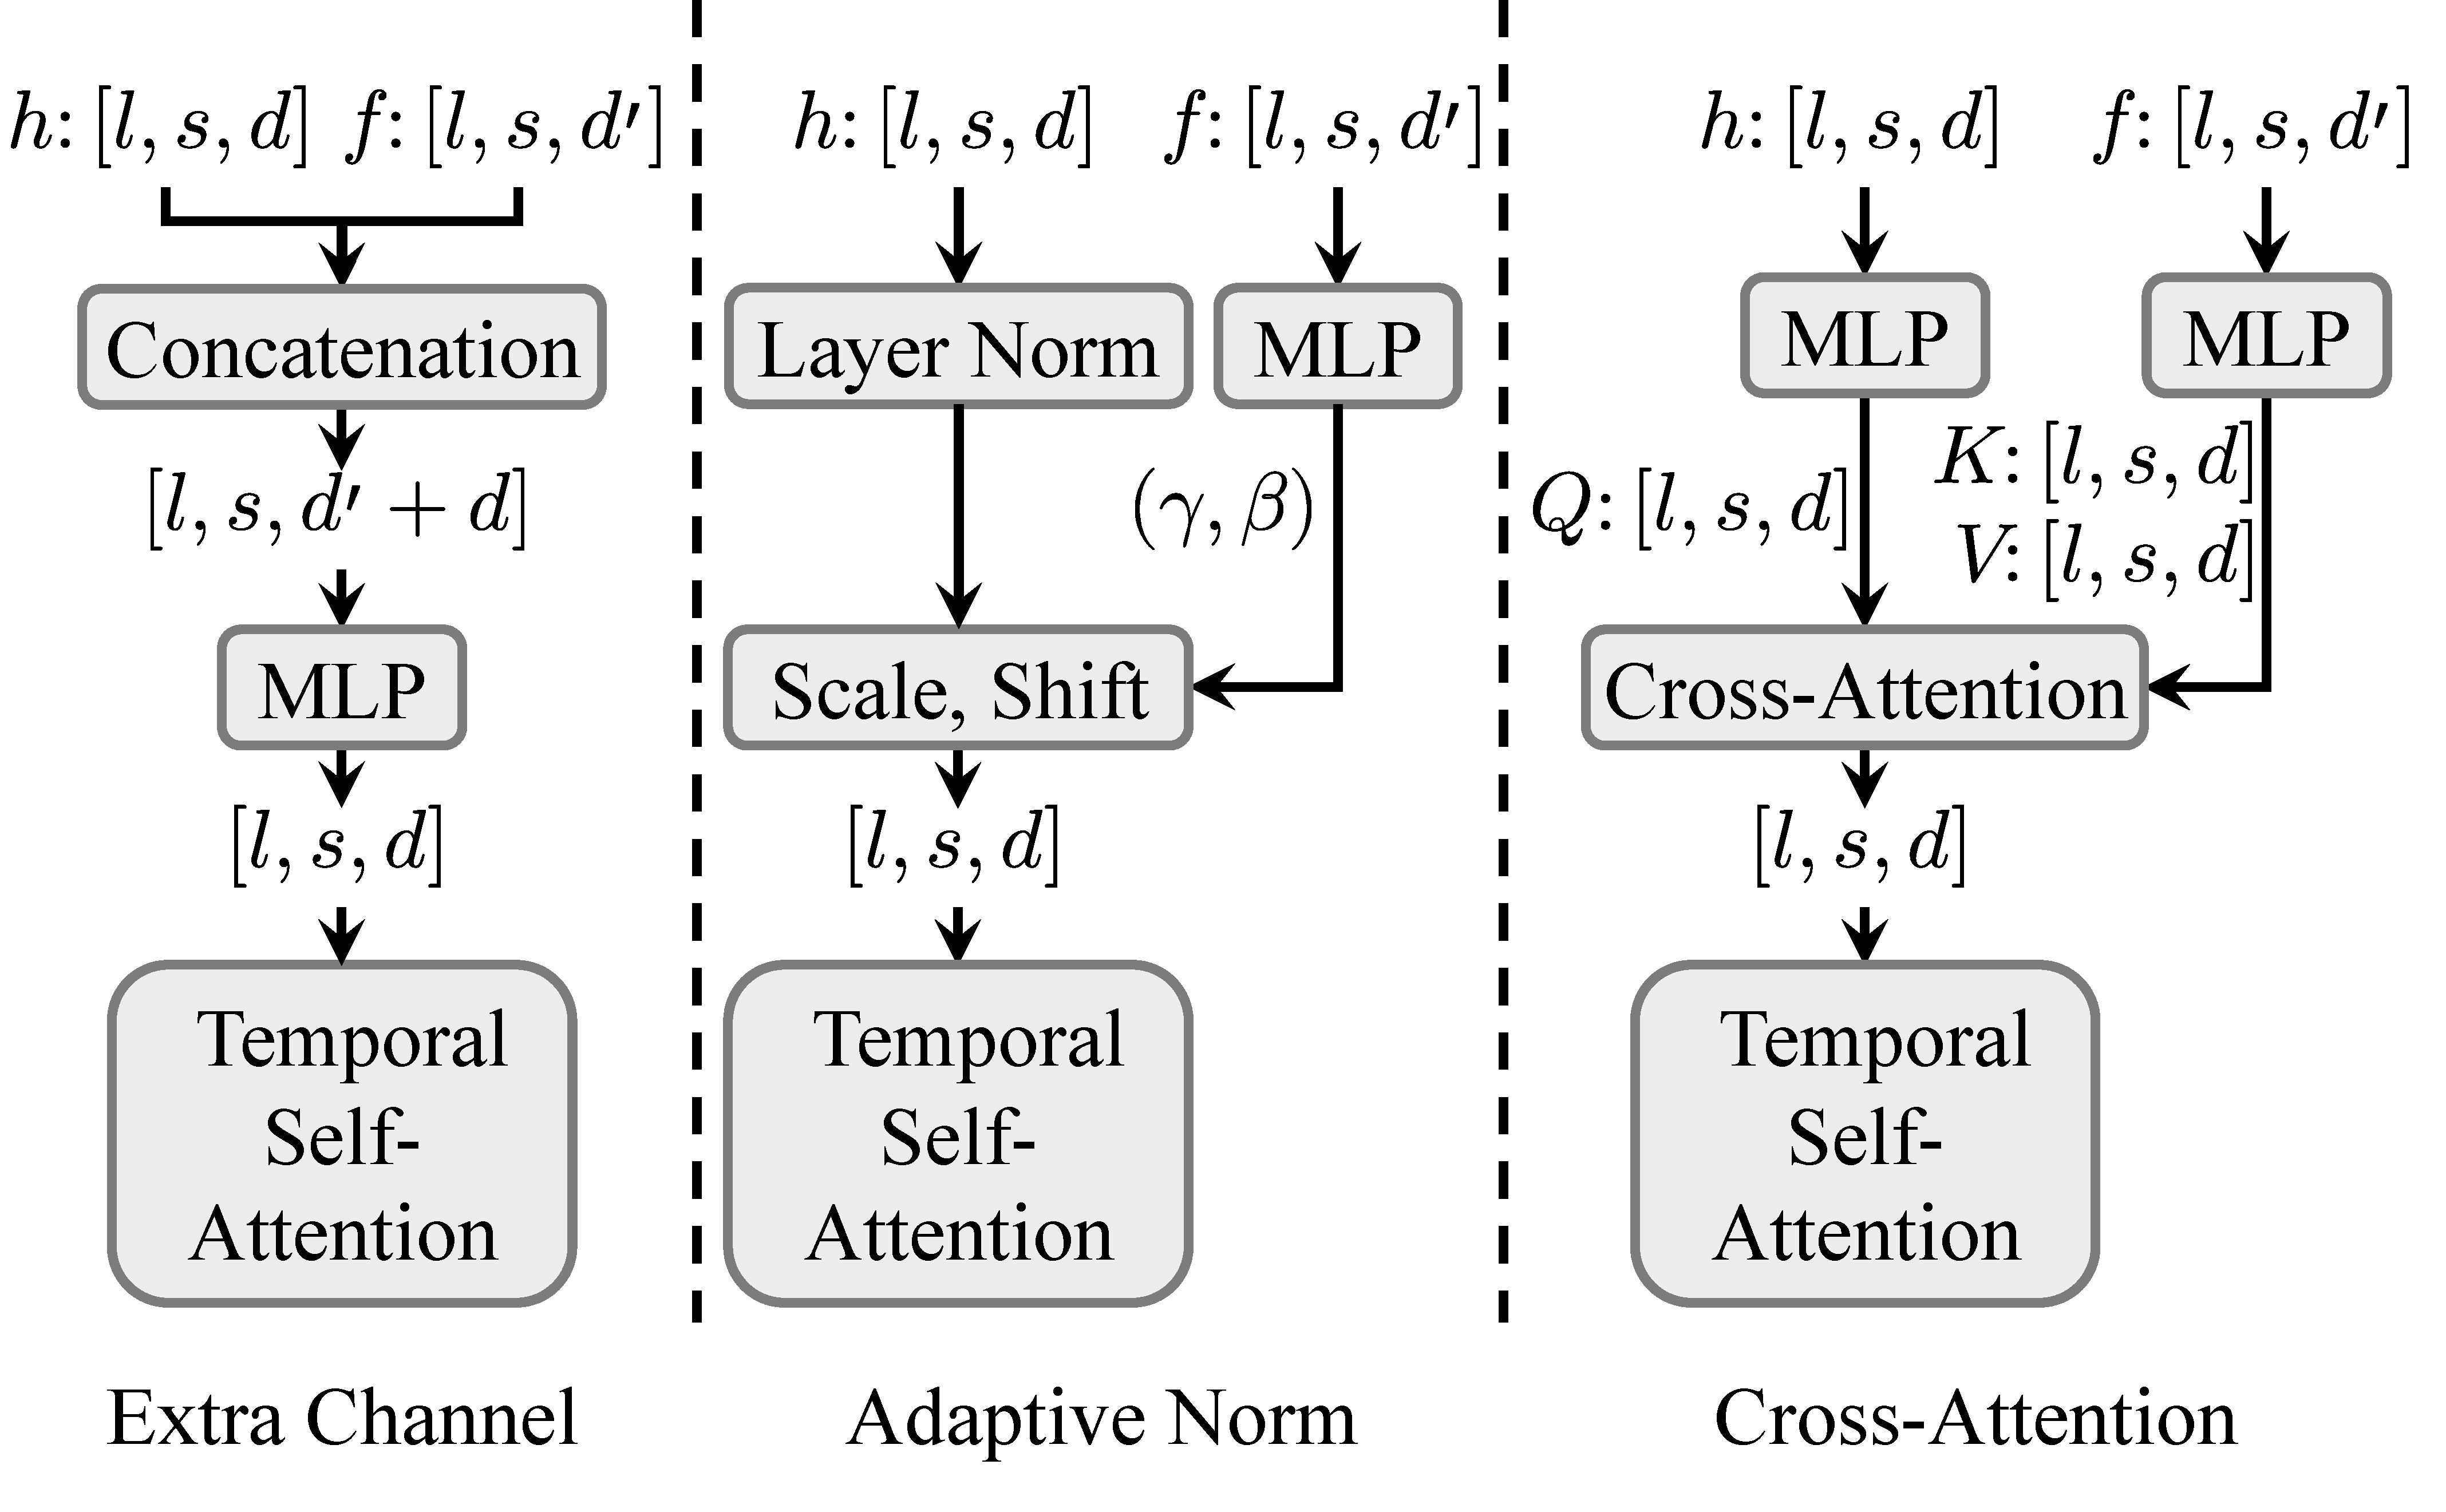
\includegraphics[width=0.47\textwidth]{images/fuser.pdf}
    \caption{
        Different designs of the Motion-guidance Fuser for incorporating trajectory conditioning. Adaptive Norm demonstrates the best performance.
    }
    \label{fig:4}   
\end{figure}

\begin{itemize}[label=-]
\item Extra channel connections. Denote $h_i \in \mathbb{R}^{l \times s \times d} $ as the resultant output from the $i$-$th$ block of the ST-DiT. Following the widespread use of concatenation in GAN-based LVDM, the motion patches are simply concatenated with the previous hidden state $h_{i-1}$ along the channel dimension. An additional MLP is then added to maintain the same latent size:
\begin{equation}
h_{i} = \mathrm{MLP}~([h_{i-1}, f_i]) + h_{i-1},
\end{equation}
\item Adaptive Norm layer. Inspired by the adaptive normalization layers employed in GANs, we initially convert $f_i$ into scale $\gamma_{i}$ and shift $\beta_{i}$ by adding two zero-initialized convolution layers into the ST-DiT block. Subsequently, $\gamma_{i}$ and $\beta_{i}$ are integrated into $h_i$ through a straightforward linear projection:
\begin{equation}
h_{i} = \gamma_{i} \cdot h_{i-1} + \beta_{i} + h_{i-1},
\end{equation}

\item Cross-Attention layer. The ST-DiT block has been modified to include an additional Cross-Attention layer following the SSA or TSA, with the motion patches serving as the key and value to integrate with the hidden state h: 

\begin{equation}
h_{i} = \mathrm{CrossAttn}~([h_{i-1}, f_i]) + h_{i-1},
\end{equation}
\end{itemize}

%We experiment with three types of fusion architectures, finding that the adaptive norm demonstrates the best generation performance and compute efficiency. 

We evaluate three types of fusion architectures and find that the adaptive norm yields the best performance and computational efficiency. For the remainder of the paper, MGF employs the adaptive norm layer unless otherwise specified.


% \begin{table*}[]\footnotesize
% \setlength{\tabcolsep}{1.6pt}
% \renewcommand{\arraystretch}{1.1}
% \centering
% \begin{tabular}{c|ccc|ccc|ccc}
% \hline
% \multirow{2}{*}{Method} & \multicolumn{3}{c|}{FVD~($\downarrow$)} & \multicolumn{3}{c|}{CLIPSIM~($\uparrow$)} & \multicolumn{3}{c}{TrajError~($\downarrow$)} \\ \cline{2-10}
%                         & 16-frame    & 64-frame    & 128-frame    & 16-frame     & 64-frame     & 128-frame     & 16-frame        & 64-frame        & 128-frame        \\ \hline
% VideoComposer~\cite{wang2023videocomposer}           & 529    & 668    & 856   & 0.2335  & 0.2284  & 0.2236  & 15.11      & 29.14      & 58.76      \\
% DragNUWA~\cite{yin2023dragnuwa}                & 475    & 593    & 784    & 0.2385  & 0.2341  & 0.2305  & 10.04       & 17.33      & 41.25       \\
% AnimateAnything~\cite{DBLP:journals/corr/abs-2311-12886}         & 487    & 602    & 775   & 0.2399  & 0.2342  & 0.2313  & 13.39      & 27.28      & 51.33       \\
% TrailBlazer~\cite{DBLP:journals/corr/abs-2401-00896}             & 459    & 581    & 756    & 0.2403  & 0.2351  & 0.2322  & 11.68       & 19.47      & 44.10      \\
% MotionCtrl~\cite{wang2024motionctrl}              & 463    & 572    & 731    & 0.2412  & 0.2376  & 0.2331  & 9.42       & 16.46      & 38.39       \\
% Ours                    & \textbf{438}    & \textbf{460}    & \textbf{494}    & \textbf{0.2447}  & \textbf{0.2435}  & \textbf{0.2418}  & \textbf{7.23}       & \textbf{8.45}      & \textbf{11.72}       \\ \hline
% \end{tabular}
% \caption{Quantitative comparisons with state-of-the-art motion-controllable video generation models. As the number of generated frames increases, Tora demonstrates a growing performance advantage over the UNet-based methods, maintaining a high degree of stability in trajectory control.}
% \label{tab1}
% \end{table*}



\subsection{Data Processing and Training Strategy}
%To obtain fine-grained control using arbitrary trajectories, text, images, or their combinations, we propose various training strategies for different condition injections.

\noindent \textbf{Data Processing}. We employ a structured data processing method to obtain high-quality training videos with consistent object motion. Initially, raw videos are segmented into shorter clips based on scene detection\footnote{https://github.com/Breakthrough/PySceneDetect}. Subsequently, we remove invalid videos, such as those with encoding errors, zero duration, or low resolution. Furthermore, we utilize aesthetic\footnote{https://github.com/christophschuhmann/improved-aesthetic-predictor} and optical flow scores~\cite{DBLP:journals/pami/XuZCRYTG23} to filter out low-quality videos. To concentrate on the motion of primary objects, we implement camera motion filtering, using results from motion segmentation~\cite{DBLP:conf/eccv/ZhaoLGWL22} and camera detection to exclude instances predominantly exhibiting camera movement. Dramatic object motions in certain videos can lead to significant optical flow deviations, which may interfere with trajectory training. To address this, we retain these videos based on a probability of $(1 - flow\_score / 100)$.  For eligible videos, we generate captions using the PLLaVA model~\cite{DBLP:journals/corr/abs-2404-16994}. During inference, we utilize GPT-4o~\cite{DBLP:journals/corr/abs-2303-08774} to refine prompts, ensuring alignment with training process. 
%More detailed information can be found in the supplementary materials.

\noindent \textbf{Motion condition training}. Inspired by DragNUWA and MotionCtrl, we adopt a two-stage training approach for trajectory learning. In the first stage, we extract dense optical flow \cite{DBLP:journals/pami/XuZCRYTG23} from the training video as the trajectory, providing richer information to enhance motion learning. In the second stage, we adjust the model from complete optical flow to more user-friendly trajectories by randomly selecting 1 to $N$  object trajectories based on motion segmentation results and flow scores. To improve the scattered nature of sparse trajectories, we apply a Gaussian filter for refinement. After completing the two-stage training, Tora facilitates flexible motion control using arbitrary trajectories.

\noindent \textbf{Image condition training}. We employ a mask strategy to support visual conditioning. Specifically, we randomly unmask frames during training, ensuring that the video patches of unmasked frames are not subjected to any noise.
%This enables our Tora model to seamlessly integrate text, images, and trajectories into a unified model.


%For Tora, it is essential that training videos are annotated with captions and movement trajectories. To fulfill this requirement, we employ a structured data processing method. Initially, raw videos are segmented into shorter clips based on scene detection. Subsequently, these clips are evaluated using aesthetic scores and flow scores. To better obtain object trajectories,  We employ the results of motion segmentation and camera detection to remove instances that primarily contain camera movement. The details of the filtering threshold can be found in the supplementary materials. Additionally, dramatic object motions in some videos can cause significant optical flow deviations, interfering with trajectory training. Consequently, we retain these videos with a probability of $(1 - score / 100)$. For eligible videos, we generate captions using the PLLaVA model~\cite{DBLP:journals/corr/abs-2404-16994}. During inference, we utilize GPT-4o~\cite{DBLP:journals/corr/abs-2303-08774} to refine prompts, ensuring alignment with the training process for enhanced consistency. https://github.com/Breakthrough/PySceneDetect
